\subsection{Presentation}

\textbf{Graph theory} is a branch of mathematics that deals with the study of graphs,
which are mathematical structures used to model pairwise relationships between
objects. Graphs consist of vertices (also called nodes) that are connected by
edges. The edges can be either directed (one-way) or undirected (two-way) and can
also have a weight. \newline

\textbf{The Maximum Edge Weight Clique} (MEWC) problem is an optimization problem
in graph theory that asks for the clique (a subset of vertices, all adjacent to
one another) with the maximum total weight in an edge-weighted undirected graph.
In the MEWC problem, each edge has a weight, and the weight of a clique is the
sum of the weights of its edges. The goal is to find a clique with the maximum
possible weight. \newline

Now, the MEWC problem is \textbf{NP-hard}, which means that it is not possible
to find an efficient algorithm to solve it in polynomial time or that this problem
is at least as hard as the hardest problems in NP. It is also the generalization
of the Maximum Clique Problem (MCP), which is the special case where all edges
have the same weight. \newline

\begin{minipage}{0.5\textwidth}
    For example, the following graph $G=(V,E)$ has for its set of vertices
    $V=\{1,2,3,4,5,6\}$ and for its set of edges
    $E=\{(1,2),(1,5),(2,3),(2,5),(3,4),(4,5),(4,6)\}$.
    As we can see, the \textcolor{red}{red} edges $\{(1,2),(1,5),(2,5)\}$ form a 
    clique of size 3 and the other colored edges are each cliques of size 1. 
    We can also easily deduct that the maximum clique of G is the 
    \textcolor{red}{red} clique of size 3.
\end{minipage}
\begin{minipage}{0.5\textwidth}
    \begin{figure}[H]
        \centering
        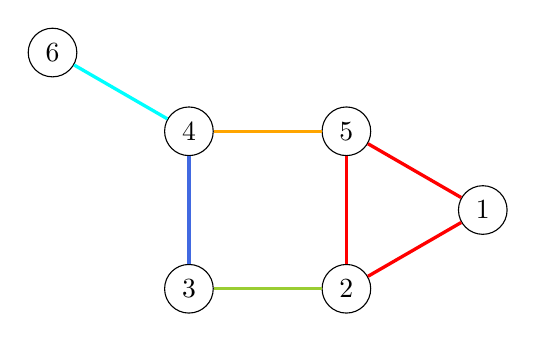
\begin{tikzpicture}[node distance=2cm, nodes={circle,draw}]
            \node (1) {1};
            \node (2) at ([shift=(210:2)] 1) {2};
            \node (3) [left of=2] {3};
            \node (4) [above of=3] {4};
            \node (5) [above of=2] {5};
            \node (6) at ([shift=(150:2)] 4) {6};

            \draw[Red, very thick] (1) -- (2);
            \draw[Red, very thick] (1) -- (5);
            \draw[YellowGreen, very thick] (2) -- (3);
            \draw[Red, very thick] (2) -- (5);
            \draw[RoyalBlue, very thick] (3) -- (4);
            \draw[Orange, very thick] (4) -- (5);
            \draw[Cyan, very thick] (4) -- (6);
        \end{tikzpicture}
        \caption{Basic graph example}
        \label{fig:basic-graph-example}
    \end{figure}
\end{minipage} \\ \\

The MEWC problem can be used to model various types of real-world situations where
the goal is to find a subset of objects with the maximum total weight, and the
objects are connected by weighted edges. Here are a few examples of such situations:

\begin{itemize}
    \item \textbf{Network design}: In a communication network, the MEWC problem
          can be used to find the optimal subset of devices (vertices) to include in
          the network, such that the total cost of communication between the devices
          (edges) is maximum.
    \item \textbf{Protein interaction}: In biology, the MEWC problem can be used
          to find the optimal subset of proteins (vertices) in a protein-protein
          interaction network, such that the total interaction strength (edges)
          between the proteins is maximum.
    \item \textbf{Social network analysis}: In a social network, the MEWC problem
          can be used to find the optimal subset of individuals (vertices) with
          the maximum total relationship strength (edges) between them.
\end{itemize}